\section{Функции обработчика прерывания от системного таймера в защищенном режиме в Unix}

\begin{enumerate}
	\item по тику
	      \begin{itemize}
		      \item инкрементирует счетчик тиков аппаратного таймера;
		      \item инкрементирует часы и другие таймеры системы;
		      \item декрементирует счетчик времени до отправления на выполнение отложенного вызова;
		      \item инкрементирует счетчик использования процессора текущим процессом;
		      \item декременирует квант текущего потока.
	      \end{itemize}
	\item по главному тику
	      \begin{itemize}
		      \item регистрирует отложенные вызовы (см. пояснения ниже) функций , относящиеся к работе планировщика;
		      \item регистрирует отложенный вызова (см. пояснения ниже) процедуры wakeup, которая
		            перемещает дескрипторы процессов из очереди «спящих» в
					очередь «готовых к выполнению»;

Так, в системе SVR4 можно зарегистрировать отложенный вызов с помощью
\texttt{timeout(void (*fn)(), caddr\_t arg, long delta);} где \texttt{fn()} - функция, которую
необходимо запустить, \texttt{arg} - аргументы, которые получит \texttt{fn()}, \texttt{delta} - временной
интервал (выраженный в тиках процессора), через который \texttt{fn} должна быть вызвана 
		      \item декрементирует счетчик времени, оставшегося до отправления одного из
		            сигналов: 
		            \begin{itemize}
			            \item SIGALARM - сигнал, посылаемый процессу по истечении времени;
			            \item SIGPROF - сигнал, посылаемый процессу по истечении времени заданном в таймере профилирования;
			            \item SIGVTALARM - сигнал, посылаемый процессу по истечении времени, заданного в «виртуальном» таймере.
		            \end{itemize}
	      \end{itemize}
	\item по кванту
	      \begin{itemize}
		      \item посылает текущему процессу сигнала SIGXCPU, если он
		            израсходовал выделенный ему квант процессорного времени.
	      \end{itemize}
\end{enumerate}

% \begin{figure}[ht!]
% 	\centering{
% 		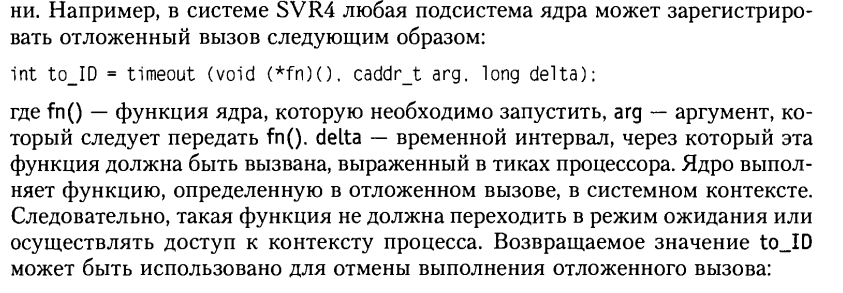
\includegraphics[width=0.9\textwidth]{img/7.png}
% 		\caption{Регистрация отложенных вызовов в SVR4.}
% 		\label{img:ref7}}
% \end{figure}

\section{Функции обработчика прерывания от системного таймера в защищенном режиме в Windows}

\begin{enumerate}
	\item по тику
	      \begin{itemize}
		      \item инкрементирует счётчик системного времени;
		      \item декрементирует остаток кванта текущего потока;
		      \item декрементирует счетчик отложенных задач;
		      \item ставит в очередь DPC объект диспетчера настройки баланса
		            (этот диспетчер активизируется каждую секунду для возможной инициации событий,
		            связанных с планированием и управлением памятью).
	      \end{itemize}
	\item по главному тику
	      \begin{itemize}
		      \item Возвращает задействованный в системе объект ''событие'', который ожидает диспетчер настройки баланса.
	      \end{itemize}
	\item по кванту
	      \begin{itemize}
		      \item инициализирует диспетчеризацию потоков путем постановки соответствующего объекта в очередь DPC.
	      \end{itemize}
\end{enumerate}

\section{Пересчет динамических приоритетов.}

Только \textbf{приоритеты пользовательских
	процессов} могут динамически пересчитываться.

\section{Пересчет динамических приоритетов в Unix.}

Вытесняемое ядро означает, что процесс в режиме ядра 
может быть вытеснен более приоритетным процессом в режиме ядра.
Это сделано для того, 
чтобы система могла обслуживать процессы реального времени,
такие как:

\begin{enumerate}
	\item аудио;
	\item видео.
\end{enumerate}

В современных системах UNIX/Linux ядро является вытесняемым.

Приоритет задается любым целым числом, лежащим в диапазоне от 0 до 127. 
Чем меньше такое число, тем выше приоритет. 
Приоритеты от 0 до 49 зарезервированы для ядра, они а являются фиксированными величинами
Прикладные процессы могут обладать приоритетом в диапазоне 50-127.
В первую очередь выполняются процессы с большим приоритетом,
а процессы с одинаковыми приоритетами выполняются в течении кванта
времени циклически друг за другом. 
На рисунке \ref{img:ref1} приведены поля структуры \textit{рrос},
относящиеся к приоритетам.

\begin{figure}[ht!]
	\centering{
		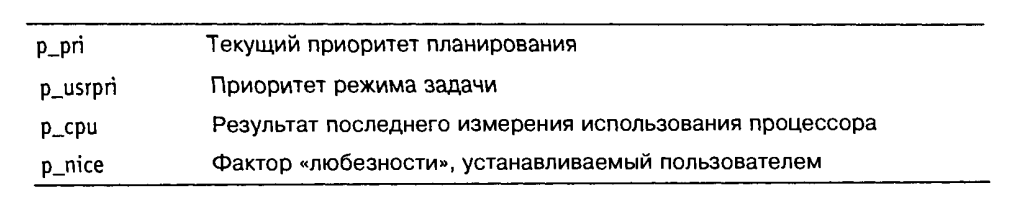
\includegraphics[width=0.9\textwidth]{img/1.png}
		\caption{Поля структуры \textit{рrос}, относящиеся к приоритетам}
		\label{img:ref1}}
\end{figure}

Планировщик использует p\_pri для принятия решения о том,
какой процесс направить на выполнение.
У процесса, находящегося в режиме задачи, значения p\_pri и p\_usrpri идентичны.
Значение текущего приоритета p\_pri может быть повышено планировщиком для выполнения процесса в режиме ядра. 
В этом случае p\_usrpri будет использоваться для хранения приоритета, который будет назначен процессу
при возврате в режим задачи. 
Фактор любезности – целое число в диапазоне от 0 до 39 со значением
20 по умолчанию. Увеличение фактора любезности приводит к уменьшению 
приоритета процесса. Фактор любезности процесса может быть
изменен суперпользователем с помощью системного вызова nice.
При создании процесса поле p\_cpu инициализируется нулем. 
На каждом тике обработчик 
таймера увеличивает поле p\_cpu текущего процесса на единицу,
до максимального значения, 
равного 127.

Ядро системы связывает приоритет сна с событием или ожидаемым ресурсом,
из-за которого процесс может блокироваться. 
Когда процесс просыпается после блокирования в системном вызове,
ядро устанавливает в поле p\_pri приоритет сна – значение приоритета
из диапазона от 0 до 49, зависящее от события или ресурса
по которому произошла блокировка. 
На рисунке \ref{img:ref2} показано 
событие и связанное с ним значение приоритета сна 
в системе 4.3BSD 

\begin{figure}[ht!]
	\centering{
		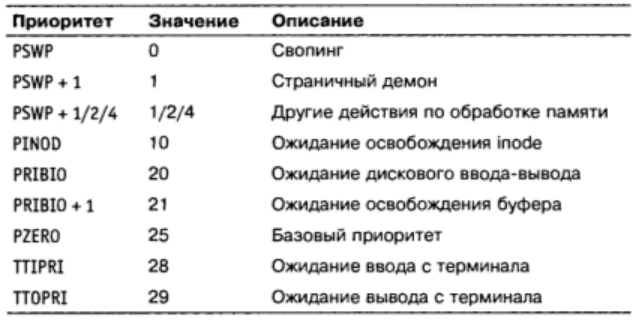
\includegraphics[width=0.9\textwidth]{img/2.png}
		\caption{Системные приоритеты сна}
		\label{img:ref2}}
\end{figure}

Каждую секунду, обработчик прерывания 
инициализирует отложенный вызов процедуры
schedcpu(), которая уменьшает значение p\_cpu каждого 
процесса исходя из фактора ''полураспада'', который рассчитывается по формуле \ref{eq:ref1}, где
\textit{load\_average} - это среднее количество процессов, находящихся в состоянии готовности к выполнению, за последнюю секунду.

\begin{equation}
	\label{eq:ref1}
	decay = \frac{2 \cdot load\_average}{2 \cdot load\_average + 1}
\end{equation}

Процедура schedcpu() пересчитывает приоритеты для режима задачи
всех процессов по формуле \ref{eq:ref2}, где \textit{PUSER} - базовый приоритет в режиме задачи, равный 50.

\begin{equation}
	\label{eq:ref2}
	p\_usrpri = PUSER + \frac{p\_cpu}{2} + 2 \cdot p\_nice
\end{equation}

В результате, если процесс в последний раз, т.е. до вытеснения другим
процессом, использовал большое количество процессорного времени, его
р\_срu будет увеличен. Это приведет к росту значения p\_usrpri и,
следовательно, к понижению приоритета. 
Чем дольше процесс простаивает в очереди на выполнение,
тем больше фактор полураспада уменьшает его
р\_срu, что приводит к повышению его приоритета. Такая схема
предотвращает бесконечное откладывание низкоприоритетных процессов
по вине операционной системы.
Ее применения предпочтительно процессам, осуществляющим много
операций ввода-вывода, в противоположность процессам, производящим
много вычислений.

\section{Пересчет динамических приоритетов в Windows.}

В Windows при создании процесса, ему назначается базовый приоритет.
Относительно базового приоритета процесса потоку назначается относительный приоритет.

Планирование осуществляется на основании приоритетов потоков, готовых к выполнению.
В Windows поток с более низким приоритетом вытесняется планировщиком, когда поток 
с более высоким приоритетом становится готовым к выполнению.
Диспетчер настройки баланса сканирует очередь готовых потоков раз в секунду и,
если обнаружены потоки, ожидающие выполнения более 4
секунд, диспетчер настройки баланса повышает их приоритет до 15. 
Как только квант истекает, приоритет потока снижается до базового приоритета.
Если поток не был завершен за квант времени или был вытеснен потоком с более высоким приоритетом, то после снижения приоритета поток
возвращается в очередь готовых потоков. 
Диспетчер настройки баланса сканирует лишь 16 готовых потоков
и повышает приоритет не более чем у 10 потоков за один проход.
При следующем проходе сканирование возобновляется
с того места, где оно было прервано в прошлый раз.\
Наличие 10 потоков, приоритет которых следует повысить,
свидетельствует о необычно высокой загруженности системы.

Windows использует 32 уровня приоритета (рисунок \ref{img:ref3}), от 0 до 31. Эти значения
разбиваются на части следующим образом:

\begin{itemize}
	\item шестнадцать уровней реального времени (от 16 до 31);
	\item шестнадцать изменяющихся уровней (от 0 до 15), из которых
	      уровень 0 зарезервирован для потока обнуления страниц.
\end{itemize}


\begin{figure}[ht!]
	\centering{
		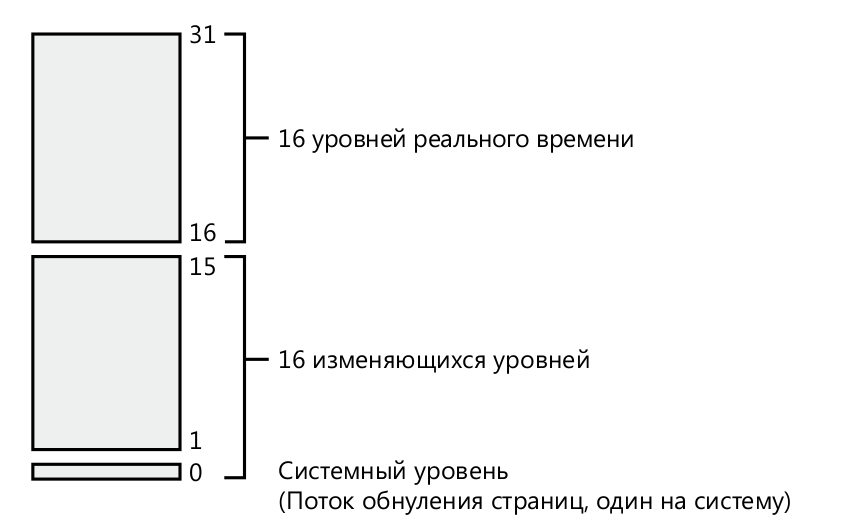
\includegraphics[width=0.9\textwidth]{img/3.png}
		\caption{Уровни приоритета потоков}
		\label{img:ref3}}
\end{figure}

Уровни приоритета потоков назначаются исходя из двух разных позиций:
одной от Windows API и другой от ядра Windows. 
Сначала Windows API систематизирует процессы по классу приоритета,
который им присваивается при создании: 
Реального времени — Real-time (4), Высокий — High (3),
Выше обычного — Above Normal (7), Обычный — Normal (2), Ниже обычного —
Below Normal (5) и Простоя — Idle (1).

Затем назначается относительный приоритет отдельных потоков внутри этих
процессов. Здесь номера представляют изменение приоритета, применяющееся
к базовому приоритету процесса: 
Критичный по времени — Time-critical (15),
Наивысший — Highest (2), Выше обычного — Above-normal (1), Обычный —
Normal (0), Ниже обычного — Below-normal (–1), Самый низший — Lowest (–2)
и Простоя — Idle (–15).

Исходный базовый приоритет потока наследуется от базового приоритета процесса. Процесс по умолчанию наследует свой базовый приоритет у
того процесса, который его создал.
Соответствие между приоритетами Windows API и ядра системы приведено
на рисунке \ref{img:ref4}.

\begin{figure}[ht!]
	\centering{
		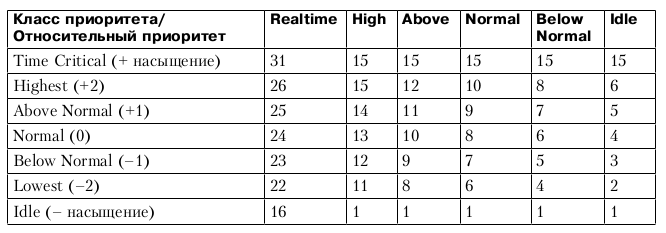
\includegraphics[width=0.9\textwidth]{img/4.png}
		\caption{Соответствие между приоритетами Windows API и ядра Windows}
		\label{img:ref4}}
\end{figure}

Текущий приоритет потока в динамическом диапазоне --- от 1 до 15 --- может быть повышен планировщиком вследствие следующих причин:

\begin{itemize}
	\item повышение вследствие событие планировщика или диспетчера(сокращение
	      задержек);
	\item повышение приоритета владельца блокировки;
	\item повышение приоритета после завершения ввода/вывода (сокращение задержек) (рисунок \ref{img:ref5});
	\item повышение приоритета вследствие ввода из пользовательского интерфейса(сокращение
	      задержек и времени отклика);
	\item повышение приоритета вследствие длительного ожидания ресурса исполняющей системы(предотвращение зависания);
	\item повышение вследствие ожидания объекта ядра;
	\item повышение приоритета в случае, когда готовый к выполнению поток не был запущен в течение длительного времени (предотвращение зависания и смены приоритетов);
	\item повышение приоритета проигрывания мультимедиа службой планировщика \texttt{MMCSS}.
\end{itemize}

\begin{figure}[ht!]
	\centering{
		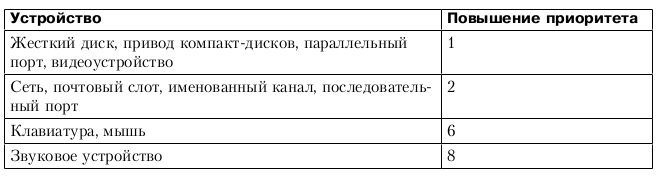
\includegraphics[width=0.9\textwidth]{img/5.png}
		\caption{Рекомендуемые значения повышения приоритета}
		\label{img:ref5}}
\end{figure}

\section{MMCSS.}

Повышение приоритета проигрывания мультимедиа обычно управляется
службой пользовательского режима, которая называется службой планировщика 
класса мультимедиа — MultiMedia Class Scheduler Service (MMCSS).
MMCSS работает с вполне определенными задачами, включая следующие:

\begin{itemize}
	\item аудио;
	\item захват;
	\item распределение;
	\item игры;
	\item проигрывание;
	\item аудио профессионального качества;
	\item задачи администратора многооконного режима.
\end{itemize}

В свою очередь, каждая из этих задач включает информацию о свойствах, отличающих
их друг от друга. Одно из наиболее важных свойств для планирования
потоков называется категорией планирования — Scheduling Category, которое
является первичным фактором, определяющим приоритет потоков, зарегистрированных
с MMCSS. На рисунке \ref{img:ref6} показаны различные категории планирования.

Механизм, положенный в основу MMCSS, повышает приоритет потоков
внутри зарегистрированного процесса до уровня, соответствующего их категории
планирования.

\begin{figure}[ht!]
	\centering{
		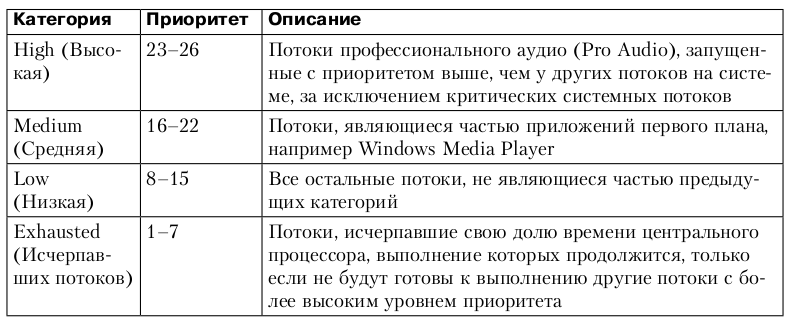
\includegraphics[width=0.9\textwidth]{img/6.png}
		\caption{Категории планирования}
		\label{img:ref6}}
\end{figure}

Затем он снижает категорию этих потоков до Exhausted,
чтобы другие, не относящиеся к мультимедийным
приложениям потоки, также могли получить ресурс.

\newpage

\section{Вывод}

Несмотря на то, что Windows и Unix разные операционные системы
обработчик системного таймера выполняет
схожие основные функции:

\begin{itemize}
	\item инициализируют отложенные действия (такие как пересчет приоритетов);
	\item выполняют декремент счетчиков времени:
	      \begin{enumerate}
		      \item часов;
		      \item таймеров;
		      \item будильников реального времени;
		      \item счетчиков времени отложенных действий.
	      \end{enumerate}
	\item уменьшает квант процессорного времени, выделенного процессу.
\end{itemize}

Обе операционные системы являются системами
разделения времени с вытеснением и динамическими приоритетами.

Приоритет пользовательского процесса в ОС Unix/Linux
может динамически пересчитываться, в зависимости от
фактора любезности, p\_cpu и базового приоритета. 
Приоритеты ядра являются фиксированными величинами.

При создании процесса в Windows, ему назначается базовый приоритет. 
Относительно базового приоритета процесса потоку назначается
относительный приоритет, таким образом у потока нет своего приоритета.
Приоритет потока пользовательского процесса может быть динамически пересчитан.

В любой системе у процесса базовый приоритет. 
Классическое ядро Unix не было многопоточным. 
Современные ядра и ядра Linux многопоточные.

\newpage

\section{Литература}

1) Вахалия. UNIX изнутри.

2) Соломон, Руссинович. Внутреннее устройство Windows.
